% -*- latex -*-
%%%%%%%%%%%%%%%%%%%%%%%%%%%%%%%%%%%%%%%%%%%%%%%%%%%%%%%%%%%%%%%%
%%%%
%%%% This TeX file is part of the course
%%%% Introduction to Scientific Programming in C++/Fortran2003
%%%% copyright 2017-2023 Victor Eijkhout eijkhout@tacc.utexas.edu
%%%%
%%%% range.tex : about iterators and ranging
%%%%
%%%%%%%%%%%%%%%%%%%%%%%%%%%%%%%%%%%%%%%%%%%%%%%%%%%%%%%%%%%%%%%%

You have seen how you can iterate over a vector
\begin{itemize}
\item by an indexed loop over the indices, and
\item with a range-based loop over the values.
\end{itemize}
There is a third way, which is actually the basic mechanism underlying
the range-based looping.
For this you need to realize that
iterating through objects such as vectors isn't simply a process
of keeping a counter that says where you are, and taking that element if needed.

Many C++ classes have an \indextermdef{iterator} subclass,
that gives a formal description of `where you are' and what you can find there.
Having iterators means that you can traverse structures that don't have
an explicit index count, but there are many other conveniences as well.

An \indexterm{iterator} is, in a metaphorical sense
a pointer to a vector element:
something that indicates a location in a container
such as a vector.
Here are some ways iterator are similar to indexes:

\begin{block}{Iterator basics}
  \begin{itemize}
  \item
    Iteratable containers have a \indexc{begin} and \indexc{end} iterator.
  \item
    The end iterator `points' just beyond the last element.
  \item The `\lstinline+*+' star operator gives the element that the iterator points to.
  \item You can increment and decrement them (for certain containers).
  \end{itemize}
  %%\snippetwithoutput{iterplusminus}{iter}{plusminus}
\end{block}

We start with a discussion of ranges that does not involve iterators,
and then we go on to the more general and basic mechanism.

\Level 0 {Ranges}
\label{sec:ranges}

The \cppstandard{20} standard contains a \indextermtt{ranges} header,
which generalizes iteratable objects into as-it-were streams,
that can be connected with \indextermp{pipe}s.

We need to introduce two new concepts.

A \indexcdef{range} is an iteratable object.
The containers of the pre-17 \ac{STL} are ranges, but
some new ones have been added.

First of all, ranges provide a clear syntax:
\begin{lstlisting}
vector data{2,3,1};
ranges::sort(data);
\end{lstlisting}
or
\verbatimsnippet{sumelem}

\begin{block}{Practical note}
  In the examples to follow we will write
\begin{lstlisting}
rng::transform
\end{lstlisting}
  and such where 
\begin{lstlisting}
#include <ranges>
namespace rng = std::ranges;
\end{lstlisting}
  However, some features are taken from the \indexterm{ranges-v3} library,
  and
\begin{lstlisting}
#include <range/v3/all.hpp>
namespace rng = ranges;
\end{lstlisting}
\end{block}

\Level 1 {Views}

A \emph{view}\index{view|see{range, view}}\index{range!view}
is somewhat similar to a range, in the sense that
you can iterate over it.
The difference is that, unlike for instance a \indexc{vector},
a view is not a completely formed object:
it is a sort of transformation of a range.

You would typically write something like:
\begin{lstlisting}
yourcontainer | someview
\end{lstlisting}
and the result of this is just as iteratable the original container.
The `view' is often a \indextermbus{range}{adaptor}, taken
from the \indexc{views} namespace. For instance:
\begin{lstlisting}
myvector | views::drop(5)
\end{lstlisting}
which acts as if you omitted the first~5 elements from your vector.

A~view doesn't own any data, and any elements you view in it get formed
as you iterate over it.
This is sometimes called \indexterm{lazy evaluation}
or \indexterm{lazy execution}.
Stated differently, its elements are constructed
as they are being requested by the iteration over the view.

Views are composable: you can take one view, and pipe it into another one.
If you need the resulting object, rather than the elements as a stream,
you can call
\begin{lstlisting}
auto newvector = myvector | views::drop(5) | to<vector<int>>();
\end{lstlisting}

First two simple examples of views:
\begin{enumerate}
\item
  one formed by \indexcdef{transform}, which applies
  a function to each element of the range or view in sequence;
\item one formed by \indexcdef{filter}, which only
  yields those elements that satisfy some boolean test.
\end{enumerate}
%% (We use an auxiliary function to turn a vector into a string.)

\snippetwithoutput{filtertransform}{range}{ft1}

Next to illustrate the composition of streams:

\snippetwithoutput{filtertransformpipe}{range}{ft2}

Let's exercise this piping of containers and views.

\begin{exercise}
  Make a vector that contains both positive and negative numbers.
  Use ranges to compute the minimum square root of the positive numbers.
  \begin{enumerate}
  \item Start with a vector of numbers;
  \item Make an iteratable view containing just the square roots of the positive numbers;
  \item Find the minimum of these roots.
  \end{enumerate}
\end{exercise}

Other available operations:
\begin{itemize}
\item dropping initial elements: \lstinline+std::views::drop+
\item reversing a vector: \lstinline+std::views::reverse+
\end{itemize}

In \cppstandard{23} some more views have been added.
We show only some of the important ones.

\begin{block}{Zipped views}
  \label{sl:range-zip}
  Zip ranges together with \lstinline{ranges::views::}\indexc{zip},
  giving a tuple:
  \snippetwithoutput{rangeszip}{ranges}{zip}
\end{block}

\begin{block}{Sliding window}
  \label{sl:range-adjacent}
  Return adjacent elements with \lstinline{ranges::views::}\indexc{adjacent},
  giving a tuple.
  \verbatimsnippet{rangeadj3}
  \begin{quote}
    Not yet available in my compiler, or in the \indextermtt{range-v3} library.
  \end{quote}
\end{block}

\Level 1 {Example: sum of squares}

For computing the sum of squares of the elements of a vector.
we can use the range \indexc{transform} method
for constructing a `lazy container' of the squares.
However, \cppstandard{20} does not have a range version
of the algorithms in \indexc{numeric} header,
such as \indexc{accumulate}.
This is fixed in \cppstandard{23}.

\verbatimsnippet{sumsquaretransform}

\Level 1 {Infinite sequences}

Since views are lazily constructed,
it is possible to have an infinite object
--~as long as you don't ask for its last element.

In the following example we make a view \lstinline{even_numbers}
that `contains' all even numbers,
and then we print only the first ten of them:
%
\snippetwithoutput{infeven}{range}{infinite}

Here we used the range version of \indexc{iota}
in the variant where only the lower bound is specified.

\Level 0 {Iterators}
\label{sec:iterator}
\label{sec:iterator-use}

Many algorithms that you saw above
have an older syntax using iterators.

\begin{lstlisting}
vector data{2,3,1};
// iterator syntax:
sort( begin(data),end(data) );
// range syntax
ranges::sort(data);
\end{lstlisting}
The \indexc{begin}~/ \indexc{end} functions
give something that acts like pointers to the start and end of the container.

Technically they are \indextermbus{iterator}{object}s,
which form a subclass of the container class.

\Level 1 {Using iterators}
\label{sec:iterator-class}

The container class has a subclass \indextermdef{iterator} that can be
used to iterate through all elements of a container. 

An \indexc{iterator} can be used outside of strictly iterating.
You can consider an iterator as a sort of `pointer into a container',
and you can move it about.

Let's look at some examples of using
the \indexcdef{begin} and \indexcdef{end} iterators.
In the following example:
\begin{itemize}
\item We first assign the \lstinline{begin} and \lstinline{end} iterators to variables;
  the begin iterator points at the first element,
  but the end iterator points just beyond the last element;
\item Given an iterator, you get the value of the corresponding element by
  applying the `star' operator to it;
\item A sort of `pointer arithmetic' can be applied to iterators.
\end{itemize}

\begin{block}{Begin and end iterator}
  \label{sl:vec-iterator}
  Use independent of looping:
  %
  \snippetwithoutput{veciterator}{stl}{iter}
\end{block}

Note that the star notation is a
\emph{unary star operator}\index{operator!unary star}
on the iterator object,
not a
\indextermbus{pointer}{dereference}:
%
\verbatimsnippet{iterderef}

\begin{block}{Ranges vs iterators}
  \label{sl:auto-iterator}
  Equivalence of range and iterator code:
  \begin{multicols}{2}
    The range code
\begin{lstlisting}
vector<int> myvector(20);
for ( auto copy_of_int : myvector )
  s += copy_of_int;
\end{lstlisting}
\columnbreak
    is actually short for:
\begin{lstlisting}
for
 ( std::vector<int>::iterator
     it=myvector.begin() ;
     it!=myvector.end() ; ++it ) {
       int copy_of_int = *it;
       s += copy_of_int ;
       }
\end{lstlisting}
  \end{multicols}
  Range iterators can be used with anything that is iteratable:\\
  vector, map, your own classes!
\end{block}

%% \begin{lstlisting}
%%   for ( auto &ref_to_int : myvector )
%%   ref_to_int = s;
%%   for ( const auto& copy_of_thing : myvector )
%%   s += copy_of_thing.f();
%% \end{lstlisting}

\begin{slide}{Vector iterator}
  \label{sl:iterate-vector}
  Range-based iteration
\begin{lstlisting}
for ( auto element : vec ) {
  cout << element;
}
\end{lstlisting}
 is syntactic sugar around iterator use:
\begin{lstlisting}
for (std::vector<int>::iterator elt_itr=vec.begin();
      elt_itr!=vec.end(); ++elt_itr) {
  element = *elt_itr;
  cout << element;
}
\end{lstlisting}
\end{slide}

Another illustration of iterators is getting the
last element of a vector:
We start by getting the value through the \lstinline{back} method.

\begin{block}{Last element by value}
  Use \indexc{back} to get the value of the last element:
  %
  \snippetwithoutput{vectorpush}{array}{vectorend}
\end{block}

Next we use the iterator mechanism.
The \indexc{end} iterator points just `beyond' the data,
so we shift it left and get its value.

\begin{block}{last element by iterator}
  Set an iterator to the last element and `dereference' it:
  %
  \snippetwithoutput[vectorend]{vectorpushiterator}{array}{vectorenditerator}
\end{block}

\Level 1 {Why still iterators, why not}

One reason that range-based algorithms are better than
iterator-based ones, is that the iterator version is prone to accidents:
\begin{lstlisting}
sort( begin(data1),end(data2) ); // OUCH
\end{lstlisting}

There are still some things that you can do with iterators that
can not be done with range-based iteration.

\begin{block}{Iterating backward}
  \label{sl:reverse-iterator}
  Reverse iteration can not be done with range-based syntax.
  
  Use general syntax with reverse iterator: \indexc{rbegin},
  \indexc{rend}.
\end{block}

\Level 1 {Forming sub-arrays}

Iterators can be used to construct a \indexc{vector}. This can
for instance be used to create a
\emph{subvector}\index{vector!subvector}.
In the simplest case, you would make a copy
of a vector using begin/end iterators:
\begin{lstlisting}
vector<int> sub( othervec.begin(),othervec.end() );
\end{lstlisting}

Note that the subvector is formed as a copy of the original elements.
Vectors completely `own' their elements. For non-owning subvectors
you would need \indexc{span}; section~\ref{sec:gsl-span}.

Some more examples. We form a subvector:
%
\snippetwithoutput[iter]{subvectorcopy}{iter}{subvectorcopy}

To demonstrate that the subvector is really a new object,
not a subset of the original vector:
\snippetwithoutput[iter]{subvectornew}{iter}{subvectornew}

\Level 1 {Vector operations through iterators}

You have already seen that the length of a vector can be
extended with the \lstinline+push_back+ method
by a single element.

With iterators other operations are possible,
such as copying, erasing, and inserting.

First we show the use of \indexcdef{copy} which takes
two iterators in one container to define the range to be copied,
and one iterator in the target container, which can be the same as the source.
The copy operation will overwrite elements in the target,
but without bound checking, so make sure there is enough space.

\begin{block}{Copy range}
  \label{sl:iter-copy}
  Copy a begin/end range of one container\\
  to an iterator in another container::
  \snippetwithoutput{itercopy}{iter}{copy}
  (No bound checking, so be careful!)
\end{block}

The erase operation \indexcdef{erase} takes two iterators,
defining the inclusive lower and exclusive upper bound
for the range to erase.

\begin{block}{Erase at/between iterators}
  \label{sl:iter-erase}
  Erase from start to before-end:
  \snippetwithoutput{vectorerase}{iter}{erase2}
  (Also erasing a single element without end iterator.)
\end{block}

The \indexcdef{insert} operation takes a target iterator
after which the insertion takes place, and
two iterators for the range that will be inserted.
This will extend the size of the target container.

\begin{block}{Insert at iterator}
  \label{sl:iter-insert}
  Insert at iterator: value, single iterator, or range:
  \snippetwithoutput{vectorinsert}{iter}{insert2}
\end{block}

\Level 2 {Indexing and iterating}

Functions that would return an array element or location,
now return iterators. For instance:
\begin{itemize}
\item \indexc{find} returns an iterator pointing to the first element
  equal to the value we are finding;
\item \indexc{max_element} returns an iterator pointing to the
  element with maximum value.
\end{itemize}

One of the arguments for range-based indexing was
that we get a simple syntax if we don't need the index.
Is it possible to use iterators and still get the index?
Yes, that's what the function \indexcdef{distance} is for.

\begin{block}{Reconstruct index}
  \label{sl:iterator-distance}
  Find `index' by getting the distance between
  two iterators:
  %
  \snippetwithoutput{vecdist}{loop}{distance}
\end{block}

\begin{slide}{Iterator arithmetic}
  \label{sl:iterator-arithmetic}
  \begin{lstlisting}
    auto first = myarray.begin();
    first += 2;
    auto last  = myarray.end();
    last  -= 2;
    myarray.erase(first,last);
  \end{lstlisting}
\end{slide}

\begin{exercise}
  Use the above vector methods to return,
  given a \lstinline+std::vector<float>+,
  the integer index of its maximum element.
\end{exercise}

\Level 0 {Algorithms using iterators}
\label{sec:algorithm}

Many simple algorithms on arrays, such as testing `there is' or `for all',
no longer have to be coded out in~C++.
They can now be done with a single
function from the \lstinline{std::}\indexheaderdef{algorithm} library.
This contains `components that C++ programs may use to perform
algorithmic operations on containers and other sequences'.

So, even if you have learned a to code a specific algorithm yourself
in the foregoing,
you should study the following algorithms,
or at least known that such algorithms exist.
It's what distinguishes a novice programmer
from an industrial-grade (for want of a better term) programmer.

\Level 1 {Test Any/all}
\label{sec:alg-iter}

First we look at some algorithms that apply a predicate
to the elements.
\begin{itemize}
\item Test if any element satisfies a condition:
  \indexcdef{any_of}.
  Note that both \lstinline{std::any_of} and
  \lstinline{std::ranges::any_of} exist.
  The same holds for the next two.
\item Test if all elements satisfy a condition:
  \indexcdef{all_of}.
\item Test if no elements satisfy a condition:
  \indexcdef{none_of}.
\item Apply an operation to all elements: \indexcdef{for_each}.
\end{itemize}

The object to which the function applies is not specified directly; 
rather, you have to specify a start
and end iterator.

(See 
chapter~\ref{ch:lambda} for the use of lambda expressions.)

As an example of applying a predicate we look at a couple of examples
of using \indexc{any_of}.
This returns true or false depending on whether the predicate is true
for any element of the container;
this uses \indexterm{short-circuit evaluation}.

\begin{block}{For any}
  \label{sl:alg-any}
  Reduction with boolean result:\\
  See if any element satisfies a test
  %
  \snippetwithoutput{algeachr}{iter}{eachr}
  %
  (Why wouldn't you use a \indexc{accumulate} reduction?)
\end{block}

\begin{block}{Any of}
  \label{sl:lambda-any}
  Here is an example using \indexc{any_of} to find
  whether a certain  element appears in a vector:
  %
  \snippetwithoutput{alganyr}{iter}{anyr}
\end{block}

Capturing the value to be tested gives:
%
\snippetwithoutput{alganyrc}{iter}{anyc}

\begin{remark}
  The previous examples rely on \cppstandard{20} ranges.
  With iterators they look like this:
  \snippetwithoutput{algany}{iter}{any}
  \snippetwithoutput{algeach}{iter}{each}
\end{remark}

\Level 1 {Apply to each}

The \indexc{for_each} algorithm applies a function to every element
of a container.
Unlike the previous algorithms, this can alter the elements.

To introduce the syntax, we look at the pointless example of
outputting each element:

%
\snippetwithoutput{printeach}{stl}{printeach}

\begin{block}{For each, very simple example}
  \label{sl:alg-each}
  Apply something to each array element:
  \snippetwithoutput{algeachr}{iter}{eachr}  
\end{block}

\begin{exercise}
  \label{ex:for-each-sum}
  Use \indexc{for_each} to sum the elements of a vector.

  Hint: the problem is how to treat the sum variable.
  Do not use a global variable!
\end{exercise}

\begin{block}{For each, with capture}
  \label{sl:alg-summing}
  Capture by reference, to update with the array elements.
  \snippetwithoutput{algsumming}{iter}{each}  
\end{block}

\Level 1 {Iterator result}

Some algorithms do not result in a value, but rather
in an iterator that points to the location of that value.
Examples: \indexc{min_element} takes a begin and end iterator,
and returns the iterator in between where the minimum element
is found.
To find the actual value, we need to `dereference'
the iterator:
%
\verbatimsnippet{minelement}

Similarly \indexc{max_element}.

\Level 1 {Mapping}

The \indexcdef{transform} algorithm applies a function to each
container element, modifying it in place:
\begin{lstlisting}
std::transform( vec, vec.begin(), [] (int i) { return i*i; } );
\end{lstlisting}

\Level 1 {Reduction}

Numerical \emph{reductions}\index{reduction} can be applied using iterators
in \indexcdef{accumulate} in the \indexc{numeric} header.
If no reduction operator is specified, a
\indextermsub{sum}{reduction}\index{sum, reduction|see{reduction, sum}}
is performed.

\begin{block}{Reduction operation}
  \label{sl:vec-accumulate}
  Default is sum reduction:
  %
  \snippetwithoutput[reduce]{vecaccumulate}{stl}{accumulate}
  %
\end{block}

Other binary \indextermsubp{arithmetic}{operator}
that can be used as \indextermbus{reduction}{operator}
are found in \indextermheader{functional}:
\begin{itemize}
\item
  \indexc{plus},
  \indexc{minus},
  \indexc{multiplies},
  \indexc{divides},
\item integers only:
  \indexc{modulus}
\item boolean:
  \indexc{logical_and}, \indexc{logical_or}  
\end{itemize}

This header also contains the unary
\indexc{negate} operator, which 
can of course not be used for reductions.

As an example of an explicitly specified reduction operator:
\begin{lstlisting}
auto p = std::accumulate
  ( x.begin(),x_end(),1.f,
    std::multiplies<float>()
  );
\end{lstlisting}
Note:
\begin{itemize}
\item that the operator is templated,
  and that it is followed by parentheses
  to become a functor, rather than a class;
\item that the accumulate function is templated,
  and it takes its type from the init value.
  Thus, in the above example, a~value of~\lstinline+1+
  would have turned this into an integer operation.
\end{itemize}

Using lambda functions (chapter~\ref{ch:lambda})
we can get more complicated effects.

\begin{block}{Reduction with supplied operator}
  \label{sl:vec-multiplies}
  Supply multiply operator:
  %
  \snippetwithoutput[reduce]{vecproduct}{stl}{product}  
\end{block}

Specific for the max reduction is \indexcdef{max_element}.
This can be called without a comparator (for numerical max),
or with a comparator for general maximum operations.
The maximum and minimum algorithms return an iterator,
rather than only the max/min value.

\begin{block}{Max reduction}
  Example: maximum relative deviation from a quantity:
\begin{lstlisting}
max_element(myvalue.begin(),myvalue.end(),
    [my_sum_of_squares] (double x,double y) -> bool {
        return fabs( (my_sum_of_squares-x)/x ) < fabs( (my_sum_of_squares-y)/y ); }
);
\end{lstlisting}
\end{block}

For more complicated lambdas used in \lstinline{accumulate},
\begin{itemize}
\item the first argument should be the reduce type,
\item the second argument should be the iterated type
\end{itemize}
In the following example we accumulate one member
of a class:

\begin{block}{Custom reduction function}
  \label{sl:reduce-icomp}
  \begin{multicols}{2}
    \verbatimsnippet{classaccumulate1}
    \columnbreak
    \verbatimsnippet{classaccumulate2}
  \end{multicols}
\end{block}

\begin{remark}
  The \indexc{accumulate} algorithm does not have a parallel version
  with an \indextermbus{execution}{policy}.
  For that, see \indexcstd{reduce} in the \indexheader{numeric} header.
\end{remark}

\Level 1 {Sorting}
\label{sec:stl:sort}

The \lstinline{algorithm} header also has a function \indexcdef{sort}.

With iterators you can easily apply this to things such as vectors:
\begin{lstlisting}
sort( myvec.begin(),myvec.end() );
\end{lstlisting}
The comparison used by default is ascending.
You can specify other compare functions:
\begin{lstlisting}
sort( myvec.begin(),myvec.end(),
      [] (int i,int) { return i>j; }
    );
\end{lstlisting}
or
\begin{lstlisting}
sort( people.begin(),people.end(),
      [] ( const Person& lhs,const Person& rhs ) {
         return lhs.name < rhs.name; }
    )
\end{lstlisting}
With iterators you can also do things like sorting a part of the vector:
\snippetwithoutput{iteratorsort}{range}{sortit}

\begin{slide}{Sorting}
  \label{sl:sort-it}
  Iterator syntax:\\
  (see later for ranges)
\begin{lstlisting}
sort( myvec.begin(),myvec.end() );
\end{lstlisting}
The comparison used by default is ascending.
You can specify other compare functions:
\begin{lstlisting}
sort( myvec.begin(),myvec.end(),
      [] (int i,int j) { return i>j; }
    );
\end{lstlisting}
\end{slide}

\Level 0 {Parallel execution policies}

The \cppstandard{17} standard added the \indextermtt{ExecutionPolicy}
concept to standard algorithms,
describing how an element of the \indexheader{algorithm} library
may be executed in parallel.

There are three choices for the \indextermbus{execution}{policy},
defined in the \indexheader{execution} header:
\begin{itemize}
\item \lstinline{std::execution::seq}: iterations may not be parallelized,
  but are indeterminedly sequenced in the evaluation thread.
\item \lstinline{std::execution::par}: iterations may be executed in parallel,
  but are indetermined sequences; 
\item \lstinline{std::execution::par_unseq}: iterations may be parallelized,
  vectorized, migrated over threads.
\item \lstinline{std::execution::unseq} (since \cppstandard{20}):
  iterations are allowed to be vectorized over.
\end{itemize}

To accomodate the indeterminate evaluation order, new
`unordered' algorithms are introduced based on
existing `ordered algorithms:
\begin{itemize}
\item \indexc{reduce}: similar \indexc{accumulate}, but unordered
  and therefore parallelizable through an \indexc{ExecutionPolicy};
\item \indexc{inclusive_scan}: similar to \indexc{partial_sum};
\item \indexc{exclusive_scan}: no ordered equivalent
\item \indexc{transform_reduce}, \indexc{transform_inclusive_scan}, \indexc{transform_exclusive_scan}.
\begin{lstlisting}
transform_reduce( execpol, first,last, init, reduce_op,transform_op );
\end{lstlisting}
\end{itemize}

Some performance measurements on these are given in
\PCSEref{sec:omp-vs-cpp-tbb}.

\Level 0 {Classification of algorithms}

(Taken from a lecture by Dietmar K\"uhl at CppCon 2017, as per its copyright notice.)

\Level 1 {Non-parallel algorithms}

\Level 2 {Order $O(1)$ algorithms}

\indexc{clamp},
\indexc{destroy_at},
\indexc{gcd},
\indexc{iter_swap},
\indexc{lcm},
\indexc{max},
\indexc{min},
\indexc{minmax},

\Level 2 {Order $O(\log n)$ algorithms}

\indexc{binary_search},
\indexc{equal_range},
\indexc{lower_bound},
\indexc{partition_point},
\indexc{pop_heap},
\indexc{push_heap},
\indexc{upperbound},

\Level 2 {Heap algorithms}

\indexc{make_heap},
\indexc{sort_heap},

\Level 2 {Permutation algorithms}

\indexc{is_permutation},
\indexc{next_permutation},
\indexc{prev_permutation},

\Level 2 {Overlapping algorithms}

\indexc{copy_backward},
\indexc{move_backward},

\Level 2 {Renamed algorithms}

\indexc{accumulate},
\indexc{partial_sum},

\Level 2 {Oddball algorithms}

\indexc{iota},
\indexc{sample},
\indexc{shuffle},

\Level 1 {Parallel algorithms}

\Level 2 {Map algorithms}

\indexc{copy},
\indexc{copy_n},
\indexc{destroy},
\indexc{destroy_n},
\indexc{fill},
\indexc{fill_n},
\indexc{for_each},
\indexc{for_each_n},
\indexc{generate},
\indexc{generate_n},
\indexc{move},
\indexc{replace},
\indexc{replace_copy},
\indexc{replace_copy_if},
\indexc{replace_if},
\indexc{reverse},
\indexc{reverse_copy},
\indexc{swap_ranges},
\indexc{transform},
\indexc{uninitalized_*},

\Level 2 {Reduce algorithms}

\indexc{adjacent_find},
\indexc{all_of},
\indexc{any_of},
\indexc{count},
\indexc{count_if},
\indexc{equal},
\indexc{find},
\indexc{find_end},
\indexc{find_first_of},
\indexc{find_if},
\indexc{find_if_not},
\indexc{includes},
\indexc{inner_product},
\indexc{is_heap},
\indexc{is_heap_until},
\indexc{is_partitioned},
\indexc{is_sorted},
\indexc{is_sorted_until},
\indexc{lexicographical_compare},
\indexc{max_element},
\indexc{min_element},
\indexc{minmax_element},
\indexc{mismatch},
\indexc{none_of},
\indexc{reduce},
\indexc{search},
\indexc{search_n},

\Level 2 {Scan algorithms}

\indexc{exclusive_scan},
\indexc{inclusive_scan},

\Level 2 {Fused algorithms}

\indexc{transform_exclusive_scan},
\indexc{transform_inclusive_scan},
\indexc{transform_reduce},

\Level 2 {Gather algorithms}

\indexc{copy_if},
\indexc{partition_copy},
\indexc{remove},
\indexc{remove_copy},
\indexc{remove_copy_if},
\indexc{remove_if},
\indexc{rotate},
\indexc{unique},
\indexc{unique_copy},

\Level 2 {Special algorithms}

\indexc{adjacent_difference},
\indexc{inplace_merge},
\indexc{merge},
\indexc{nth_element},
\indexc{partial_sort},
\indexc{partial_sort_copy},
\indexc{partition},
\indexc{rotate},
\indexc{set_difference},
\indexc{set_intersection},
\indexc{set_symmetric_difference},
\indexc{set_union},
\indexc{sort},
\indexc{stable_partition},
\indexc{stable_sort},

\Level 0 {Advanced topics}

\Level 1 {Range types}

Types of ranges:
\begin{itemize}
\item \lstinline+std::ranges::input_range+ : iterate forward at least once,
  as if you're accepting input with \lstinline{cin} and such.
\item \lstinline+std::ranges::forward_range+ : can be iterated forward,
  (for instance with plus-plus), multiple times,
  as in a \indextermsub{single-linked}{list}.
\item \lstinline+std::ranges::bidirectional_range+ : can be iterated in both
  directions, for instance with plus-plus and minus-minus.
\item \lstinline+std::ranges::random_access_range+ items can be found
  in constant time, such as with square bracket indexing.
\item \lstinline+std::ranges::contiguous_range+ : items
  are stored consecutively in memory, making address calculations possible.
\end{itemize}

\Level 1 {Make your own iterator}
\label{sec:range-iter}

You know that you can iterate over \n{vector} objects:
\begin{lstlisting}
vector<int> myvector(20);
for ( auto copy_of_int : myvector )
  s += copy_of_int;
for ( auto &ref_to_int : myvector )
  ref_to_int = s;
\end{lstlisting}
(Many other \ac{STL} classes are iteratable like this.)

This is not magic: it is possible to iterate over any class:
a \emph{class} is 
\emph{iteratable}\index{class!iteratable} that has a number of conditions satisfied.

The class needs to have:
\begin{itemize}
\item a method \indexc{begin} with prototype
\begin{lstlisting}
iteratableClass iteratableClass::begin()
\end{lstlisting}
That gives an
  object in the initial state, which we will call the `iterator object'; likewise
\item a method \indexc{end}
\begin{lstlisting}
iteratableClass iteratableClass::end()} 
\end{lstlisting}
that gives an 
  object in the final state; furthermore you need
\item an increment operator
\begin{lstlisting}
void iteratableClass::operator++()
\end{lstlisting}
that
  advances the iterator object to the next state;
\item a test
\begin{lstlisting}
bool iteratableClass::operator!=(const iteratableClass&)
\end{lstlisting}
to determine
  whether the iteration can continue; finally
\item a dereference operator 
\begin{lstlisting}
iteratableClass::operator*()
\end{lstlisting}
that takes the iterator object and returns its state.
\end{itemize}

\begin{slide}{Requirements}
  \label{sl:rangemethods}
  \begin{itemize}
  \item a method \n{iteratable iteratable::begin()}: initial state
  \item a method \n{iteratable iteratable::end()}:  final state
  \item an increment operator \n{void iteratable::operator++}: advance
  \item a test \n{bool iteratable::operator!=(const iteratable&)}
  \item a dereference operator \n{iteratable::operator*}: return state
  \end{itemize}
\end{slide}

All this was visible in pre-\cppstandard{11} iterating,
where a loop over a vector looked like:
\begin{lstlisting}
for (auto elt_ptr=vec.begin(); elt_ptr!=vec.end(); ++elt_ptr)
  element = *elt_ptr;
\end{lstlisting}
Some remarks:
\begin{itemize}
\item This is one of the very few places where you need the asterisk in C++.
  However, you're applying it to an iterator, not a pointer,
  and this is an operator you are applying.
\item As with a normal loop, the \n{end} iterator point just beyond the end
  of the vector.
\item You can do \indextermbus{pointer}{arithmetic} on iterators, as
  you can see in the \lstinline|++elt_ptr| update part of the loop header.
\end{itemize}

\Level 2 {Example 1}

\begin{block}{Simple illustration}
  \label{sl:bagdata}
  
  Let's make a class, called a \n{bag}, that models a set of integers,
  and we want to enumerate them. For simplicity sake we will make a set
  of contiguous integers:
  %
  \verbatimsnippet{bagdata}
\end{block}

\begin{block}{Internal state}
  \label{sl:bagseek}
  When you create an iterator object it will be copy of the object you
  are iterating over, except that it remembers how far it has
  searched:
  %
  \verbatimsnippet{bagseek}
\end{block}

\begin{figure}[ht]
  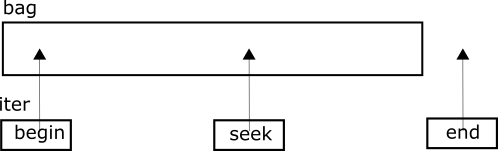
\includegraphics[scale=.8]{bagseek}
  \caption{Iterator objects into the \lstinline{bag} object}
  \label{fig:bagseek-iter}
\end{figure}

\begin{block}{Initial/final state}
  \label{sl:bagbeginend}
  The \n{begin} method gives a \n{bag} with the seek parameter
  initialized:
  %
  \verbatimsnippet{bagbeginend}
  %
  These routines are public because they are (implicitly) called by the
  client code.
\end{block}

\begin{block}{Termination test}
  \label{sl:bagtest}
  The termination test method is called on the iterator, comparing it to
  the \n{end} object:
  %
  \verbatimsnippet{bagtest}
\end{block}

\begin{block}{Dereference}
  \label{sl:bagderef}
  Finally, we need the increment method and the dereference. Both access
  the \n{seek} member:
  %
  \verbatimsnippet{bagderef}
\end{block}

\begin{block}{Use case}
  \label{sl:bagfind}

  We can iterate over our own class:
  %
  \snippetwithoutput{bagfinditer}{loop}{bagfind}

  (for this particular case, use \lstinline{std::}\indexc{any_of})
\end{block}

\begin{block}{With algorithms}
  \label{sl:bagany}

  \snippetwithoutput{bagfindany}{loop}{bagany}  
\end{block}

If we add a method \n{has} to the class:
%
\verbatimsnippet{baghastest}
%
we can call this:
%
\verbatimsnippet{bagtestcall}
%
Of course, we could have written this function
without the range-based iteration, but this implementation is
particularly elegant.

\begin{exercise}
  You can now do exercise~\ref{ex:primerange}, implementing a prime
  number generator with this mechanism.
\end{exercise}

If you think you understand \n{const}, consider that the \n{has}
method is conceptually \n{cost}. But if you add that keyword, the
compiler will complain about that use of \n{*this}, since it is
altered through the \n{begin} method.

\begin{exercise}
  \label{ex:rangeconstiter}
  Find a way to make \n{has} a \n{const} method.
\end{exercise}

\Level 2 {Example 2: iterator class}

\begin{block}{Custom iterators, 0}
  \label{sl:it-class-0}
  Recall that
  \begin{multicols}{2}
    Short hand:
\begin{lstlisting}
vector<float> v;
for ( auto e : v )
  ... e ...
\end{lstlisting}
    \columnbreak for:
\begin{lstlisting}
for ( vector<float>::iterator e=v.begin();
      e!=v.end(); e++ )
  ... *e ...
\end{lstlisting}
  \end{multicols}
  If we want 
\begin{lstlisting}
for ( auto e : my_object )
    ... e ...
\end{lstlisting}
  we need an iterator class with methods such as
  \lstinline{begin}, \lstinline{end},
  \lstinline|*| and \lstinline|++|.
\end{block}

\begin{block}{Custom iterators, 1}
  \label{sl:it-class-1}
  Ranging over a class with iterator subclass
  \begin{multicols}{2}
    Class:
    \verbatimsnippet{classwithiter}
    \columnbreak
    Main:
    \verbatimsnippet{ompcustompar}    
  \end{multicols}
  %%  \input{cppnote-custom-iterators.cut}
\end{block}

\begin{block}{Custom iterators, 2}
  \label{sl:it-class-2}
  Random-access iterator:
  \verbatimsnippet{omprandaccess}  
\end{block}

\begin{exercise}
  \label{ex:it-class}
  Write the missing iterator methods.
  Here's something to get you started.
  \verbatimsnippet{classwithiteriter}  
\end{exercise}


